\section{Resultados}
\label{sec:resultados}

Os resultados foram obtidos em duas execuções com papéis distintos. A
primeira é uma validação estrutural: utiliza as 43 carteiras do workload
apenas com carteira e perfil, sem dados externos. Ela serve para confirmar
reprodutibilidade, tratamento de lacunas e custo operacional das variantes. A
segunda é a comparação principal entre técnicas no escopo financeiro: usa
20 carteiras com enriquecimento externo por preços, fundamentos, notícias
e indicadores macroeconômicos quando disponíveis. As conclusões sobre qual
modo teve melhor desempenho, qual foi mais detalhado e qual foi mais barato são
tiradas dessa execução enriquecida, sempre comparando baselines sob a mesma
entrada.

\subsection{Validação estrutural sem enriquecimento externo}

Essa validação processou 43 carteiras em cinco baselines, totalizando
215 diagnósticos. Todos os baselines finalizaram com status \texttt{ok}, sem
falha final de execução. A Tabela~\ref{tab:classificacoes-estrutural} mostra a
distribuição das classificações produzidas por cada abordagem.

\begin{table*}[!t]
\centering
\caption{Distribuição de classificações na validação estrutural com 43 carteiras.}
\label{tab:classificacoes-estrutural}
\begin{tabular}{@{}lrrrrr@{}}
\hline\hline
Baseline & Estável & Atenção & Risco elevado & Desalinhada & Inconclusiva \\
\hline
B1   & 12 & 8 & 0 & 0 & 23 \\
B2   & 11 & 8 & 1 & 0 & 23 \\
B3   &  0 & 0 & 0 & 1 & 42 \\
B4-H &  0 & 0 & 0 & 0 & 43 \\
B4-R &  0 & 0 & 0 & 2 & 41 \\
\hline\hline
\end{tabular}
\end{table*}

O resultado mais visível é que os baselines multiagente foram mais
conservadores na ausência de dados externos. B3, B4-H e B4-R
classificaram a maioria dos casos como \textit{inconclusiva}, enquanto
B1 e B2 produziram mais classificações afirmativas. Essa assimetria não
deve ser lida automaticamente como vantagem de B1 ou B2: os prompts
proíbem inventar dados ausentes, e uma classificação inconclusiva pode
ser a resposta correta quando a entrada contém apenas tickers, pesos,
setores e perfil do usuário.

A observação importa para o objetivo do artigo. O sistema proposto não
foi desenhado para sempre emitir uma opinião forte. Ele foi desenhado
para separar diagnóstico suportado por evidência de incerteza
informacional. A alta taxa de inconclusivos nos modelos multiagente
indica, então, que a decomposição em papéis e a moderação final
expõem mais as lacunas de dados do que os baselines de agente único.

\begin{table*}[!t]
\centering
\caption{Métricas operacionais na validação estrutural com 43 carteiras. P50 e P95 são percentis de latência fim a fim.}
\label{tab:operacional-estrutural}
\begin{tabular}{@{}lrrrrrrr@{}}
\hline\hline
Baseline & OK & Chamadas & Erros & Média (s) & P50 (s) & P95 (s) & Tokens/caso \\
\hline
B1   & 43 &  43 & 0 &  16.6 &   7.1 &  68.6 &  1\,162 \\
B2   & 43 & 215 & 0 &  31.5 &  16.0 & 106.2 &  6\,147 \\
B3   & 43 & 217 & 2 &  43.1 &  34.4 & 108.2 &  9\,525 \\
B4-H & 43 & 303 & 2 &  96.3 &  68.2 & 287.6 & 21\,879 \\
B4-R & 43 & 302 & 1 & 129.7 & 113.2 & 252.6 & 21\,467 \\
\hline\hline
\end{tabular}
\end{table*}

A Tabela~\ref{tab:operacional-estrutural} mostra o custo operacional de
cada variante. B1 é o mais barato, como esperado: realiza uma única
chamada por caso. B2 sobe o custo ao usar cinco amostras de
self-consistency. B3 tem custo próximo de B2 em número de chamadas,
mas distribui o trabalho entre agentes especializados. B4-H e B4-R são
as variantes mais caras, já que incluem especialistas, debate Bull/Bear
e moderação final. O acréscimo de custo é uma limitação prática da
arquitetura e precisa ser compensado por ganhos em qualidade
estruturada, auditabilidade ou controle de incerteza.

\subsection{Comparação principal com dados externos}

Para comparar os modos em um cenário financeiro mais realista, um
subconjunto de 20 carteiras foi executado com dados coletados
automaticamente: preços e fundamentos via \texttt{yfinance}, notícias via
Brave Search API e indicadores macroeconômicos de fontes públicas quando
disponíveis. Houve uma falha pontual de B4-H em um caso da primeira rodada
enriquecida, que foi reexecutado com sucesso. A análise abaixo usa os 100
resultados finais válidos e mantém a mesma entrada para todos os baselines.

\begin{table*}[!t]
\centering
\caption{Distribuição de classificações no subconjunto enriquecido com 20 carteiras.}
\label{tab:classificacoes-enriquecido}
\begin{tabular}{@{}lrrrrr@{}}
\hline\hline
Baseline & Estável & Atenção & Risco elevado & Desalinhada & Inconclusiva \\
\hline
B1   & 3 & 17 & 0 & 0 & 0 \\
B2   & 1 & 18 & 1 & 0 & 0 \\
B3   & 0 & 14 & 6 & 0 & 0 \\
B4-H & 0 &  9 & 5 & 1 & 5 \\
B4-R & 0 &  6 & 6 & 0 & 8 \\
\hline\hline
\end{tabular}
\end{table*}

Nesse cenário, B1, B2 e B3 produzem diagnósticos conclusivos em todos os
casos. B3, B4-H e B4-R também emitem mais classificações de
\textit{risco elevado}, o que é relevante para o escopo financeiro, pois
indica maior sensibilidade a fatores negativos da carteira. B4-H e B4-R
continuam mais cautelosos que os baselines de agente único, preservando uma
fração de diagnósticos inconclusivos. A comparação central, portanto, passa
a ser entre técnicas: custo, conclusividade, detalhamento e concordância
com consenso sob a mesma entrada enriquecida.

\begin{table*}[!t]
\centering
\caption{Métricas operacionais no subconjunto enriquecido com 20 carteiras. P50 e P95 são percentis de latência fim a fim.}
\label{tab:operacional-enriquecido}
\begin{tabular}{@{}lrrrrrrr@{}}
\hline\hline
Baseline & OK & Chamadas & Erros & Média (s) & P50 (s) & P95 (s) & Tokens/caso \\
\hline
B1   & 20 &  27 &  7 &  43.4 &  23.1 & 125.1 & 15\,850 \\
B2   & 20 & 133 & 33 & 191.9 & 137.4 & 563.0 & 79\,427 \\
B3   & 20 & 142 & 22 & 212.7 & 209.0 & 367.2 & 31\,748 \\
B4-H & 20 & 199 & 39 & 354.0 & 288.9 & 753.4 & 49\,160 \\
B4-R & 20 & 178 & 18 & 297.9 & 292.2 & 443.9 & 49\,360 \\
\hline\hline
\end{tabular}
\end{table*}

O custo em tokens sobe bastante no subconjunto enriquecido porque os
prompts passam a incluir dados de mercado, fundamentos, notícias e
macroeconomia. B2 fica especialmente caro, pois replica a entrada
enriquecida em cinco amostras. B4-H e B4-R também têm custo elevado,
mas distribuem a entrada entre papéis especializados e mantêm registro
detalhado por agente. A coluna de erros representa tentativas com falha
transitória ou parsing antes de uma resposta final válida; não houve falha
final nos 100 diagnósticos do subconjunto enriquecido.

\subsection{Comparação direta entre modos de execução}

Para aproximar a análise da pergunta central do trabalho, a
Tabela~\ref{tab:comparacao-modos} compara os modos de execução em termos
de custo, detalhamento e proxy de acurácia. A acurácia proxy é calculada
como concordância com a classificação majoritária entre os cinco baselines
no mesmo caso. Dois casos empatados foram excluídos dessa métrica, deixando
18 casos no denominador. Portanto, essa coluna não deve ser interpretada
como acerto financeiro real, mas como uma medida de consistência relativa
entre abordagens que receberam a mesma entrada.

\begin{table*}[!t]
\centering
\caption{Comparação dos modos no subconjunto enriquecido. O custo em USD é uma estimativa contrafactual usando preços oficiais por token apenas para modelos com tarifa pública; tokens de modelos sem preço público são reportados à parte.}
\label{tab:comparacao-modos}
\begin{tabular}{@{}lrrrrrrr@{}}
\hline\hline
Baseline & Concl. (\%) & Acur. proxy (\%) & Fatores & Palavras & Uso proxy/caso & USD precif. & Tokens s/preço \\
\hline
B1   & 100.0 &  61.1 &  9.9 &  68.1 &  63.4 & 0.143 &      0 \\
B2   & 100.0 &  77.8 & 20.0 &  87.1 & 317.7 & 0.717 &      0 \\
B3   & 100.0 & 100.0 &  9.8 & 102.1 & 113.5 & 0.261 & 125\,884 \\
B4-H &  75.0 &  77.8 &  8.4 &  99.0 & 196.6 & 0.499 &      0 \\
B4-R &  60.0 &  61.1 &  8.8 &  93.5 & 154.7 & 0.416 & 126\,013 \\
\hline\hline
\end{tabular}
\end{table*}

\begin{figure*}[!t]
\centering
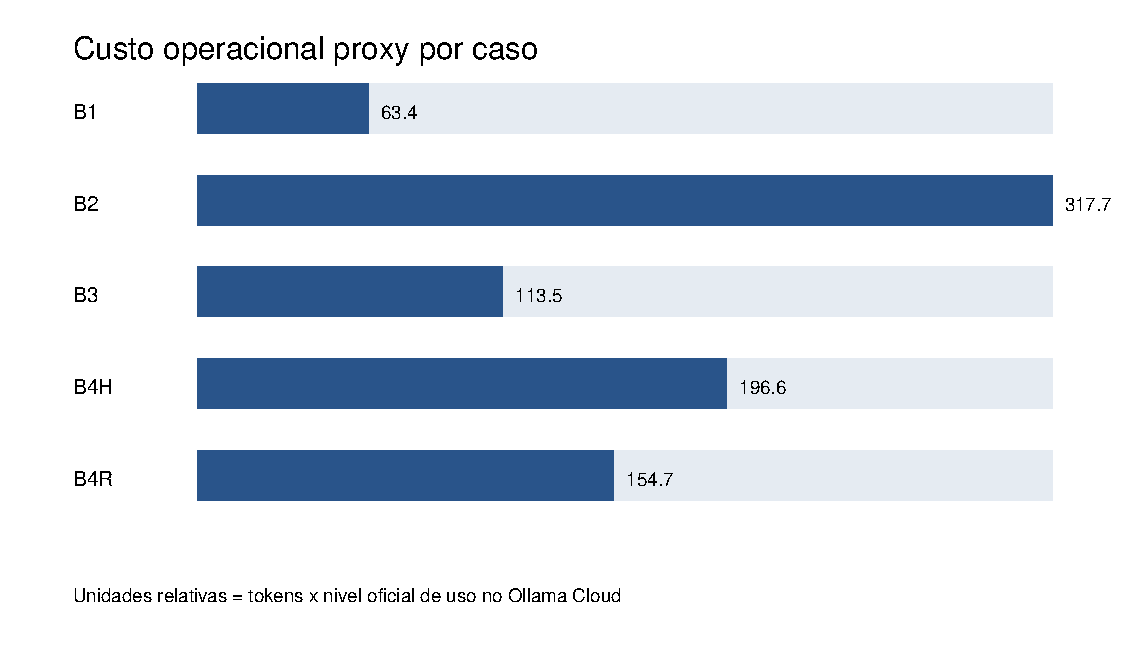
\includegraphics[width=.49\textwidth]{figures/cost_proxy.pdf}
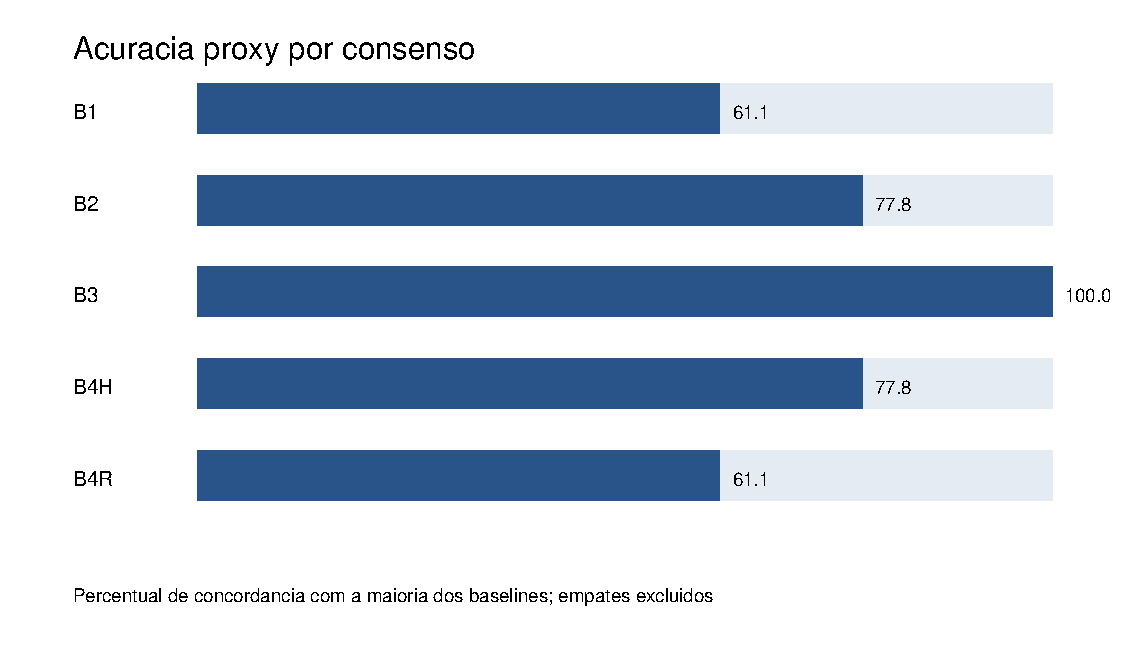
\includegraphics[width=.49\textwidth]{figures/accuracy_proxy.pdf}
\caption{Custo operacional proxy e acurácia proxy no subconjunto enriquecido. O custo proxy usa tokens multiplicados pelo nível oficial de uso do modelo no Ollama Cloud; a acurácia proxy mede concordância com o consenso dos baselines, não acerto financeiro real.}
\label{fig:custo-acuracia}
\end{figure*}

Os resultados mostram um trade-off mais claro do que a simples
distribuição de classificações. B1 é o modo mais barato e rápido, mas sua
concordância com o consenso é baixa. B2 melhora a concordância e produz a
maior quantidade média de fatores, porém é o modo mais caro em tokens e
uso proxy, pois executa cinco amostras sobre uma entrada enriquecida
longa. B3 aparece como o melhor ponto de equilíbrio nesta execução:
alcança 100\% de concordância com o consenso, mantém todos os diagnósticos
conclusivos e tem custo operacional menor que B2, B4-H e B4-R.

A comparação entre B4-H e B4-R é especialmente relevante para a proposta.
B4-R reduz o uso proxy em cerca de 21\% em relação a B4-H e também reduz
latência P95 e tentativas com erro. Isso sugere que o roteamento
heterogêneo é útil como mecanismo de controle de custo operacional. Ao
mesmo tempo, B4-R apresentou menor taxa de diagnósticos conclusivos e
menor concordância com o consenso. Assim, nesta rodada, a heterogeneidade
melhorou eficiência, mas não melhorou a proxy de acurácia.

\subsection{Discussão dos resultados}

Quatro pontos sustentam a leitura desses números. Primeiro, a arquitetura
é operacionalmente viável: todos os baselines executam sobre o mesmo
formato de entrada, produzem a mesma estrutura de saída e registram rastros
auditáveis. Segundo, a comparação financeira deve ser feita no cenário
enriquecido, porque ele fornece evidência de preço, fundamentos, notícias e
macroeconomia para todos os baselines. Terceiro, o debate adversarial ainda
não mostrou ganho claro de acurácia proxy sobre os baselines fortes. Nesta
execução, B3 superou B4-H e B4-R no trade-off entre consenso,
conclusividade e custo. Quarto, o roteamento heterogêneo de B4-R apresentou
ganho operacional em
relação a B4-H, mas esse ganho veio acompanhado de maior cautela e menor
concordância com o consenso.

Esses resultados deslocam a narrativa do artigo para uma conclusão mais
honesta. O trabalho não deve afirmar que debate multiagente é
automaticamente melhor. A evidência atual indica que a decomposição em
agentes ajuda a estruturar e auditar o diagnóstico financeiro, que B3 foi o
melhor modo de execução nesta rodada enriquecida e que o roteamento por
papel pode reduzir custo frente a uma versão homogênea. A validação de qualidade
econômica, erro factual detalhado e sensibilidade contrafactual por perfil
permanece necessária antes de afirmar superioridade financeira de B4.
